\section{Systembeschreibung} % (fold)
\label{sec:system}

\subsection{Etherpad Lite}
\label{sub:system:etherpad}

\textit{Etherpad Lite}\citeque{etherpad} ist ein kollaborativer Online-Editor.
Anwender können Textdokumente, sogenannte Pads, gemeinschaftlich und in Echtzeit online bearbeiten.
Die Oberfläche ist browserbasiert.
Innerhalb der Pads ist durch farbliche Markierung gekennzeichnet, welche Bearbeitungen von welchem Nutzer vorgenommen wurden.
Eine Instanz des Etherpad Lite ist standardmäßig offen.
Damit kann jeder Anwender Pads anlegen und bearbeiten.
Das System speichert Revisionen des Pad-Inhalts, die später abgerufen werden können.
Die Oberfläche bietet außerdem die Möglichkeit zum Export des Inhalts in verschiedene Dokumentformate sowie einen Onlinechat zur Verständigung unter den Autoren.\\
Etherpad Lite ist Open-Source und damit quelloffen und frei.

\subsection{Abgrenzung und Zielstellung}
Die Oberfläche des Etherpad Lite ist schlicht und übersichtlich gehalten.
Sie bietet benutzerrelevante Funktionen, die sich auf ein einzelnes Pad beziehen.
Administrative Funktionen, die bestimmten Benutzerkreisen vorbehalten bleiben müssen, sind auf der Oberfläche nicht implementiert.
Es gibt somit keine Möglichkeit, z.B. alle verfügbaren Pads anzuzeigen oder einzelne Pads zu löschen.\\
Es existiert eine umfangreiche HTTP-API, über die diverse Funktionen verfügbar gemacht werden.
Für die praktische Verwendung dieser API ist ein Frontend sinnvoll.\\
Das Projekt EtherApp hat zum Ziel, einen Teil der API-Funktionen abzubilden und eine App zur Administration verschiedener Etherpad-Lite-Instanzen zu entwickeln.
Das beinhaltet insbesondere folgende Funktionen:

\begin{itemize}
	\item Anzeige aller Pads
	\item Anzeige von Meta-Informationen für einzelne Pads (Benutzer online, Revisionen, Datum, …)
	\item Anlegen neuer Pads
	\item Löschen von Pads
	\item Anzeige des Pad-Inhalts
	\item Teilen der Pad-URL über soziale Dienste und E-Mail
	\item Rücksetzen des Inhalts auf ältere Revision
	\item Anzeige und Verwaltung von Gruppen
	\item Verwaltung mehrerer EPL-Instanzen und Profilverwaltung
\end{itemize}



\section{Implementation}
\label{sec:implem}
\subsection{Zugriff auf die HTTP-API}
Das EPL bietet eine umfangreiche HTTP-API\citeque{epl-httpapi} an.
Sie stellt eine Reihe von Funktionen für administrative Aufgaben bereit, die über die offene Weboberfläche nicht zur Verfügung stehen.
Der Zugriff auf die API ist nur mit einem Shared Secret (API Key) möglich, der vom Administrator festgelegt werden muss.\\
Die API gibt Antworten in JavaScript Object Notation (JSON) zurück.
Damit lassen sich Arrays oder einfache Strings gleichermaßen per HTTP übertragen.
Ein Beispiel für einen Rückgabewert aus der API ist in \autoref{lst:listallpadsjson} dargestellt (Methode \texttt{listAllPads}).
\begin{lstlisting}[caption=Rückgabewert der API zur Methode listAllPads,label=lst:listallpadsjson]
{"code":0,"message":"ok","data":{"padIDs":["interrail","interview","jabberstatusdienst,"java","Java","java2"]}}
\end{lstlisting}

Für den Zugriff auf die API existieren bereits Java-Bibliotheken, die alle API-Funktionen auf Methoden einer Java-Klasse abbilden.
Für das Projekt EtherApp kam dabei die Implementation\citeque{hollinger} von Jordan Hollinger zum Einsatz.\\
Diese Bibliothek beinhaltet eine Klasse \texttt{EPLiteClient}, welche mit den Zugangsdaten für die EPL-API initialisiert wird (siehe auch \autoref{sub:implem:eplinstanzen}).
Mit einem Objekt dieser Client-Klasse können Anfragen auf die jeweilige API durchgeführt werden, die als Java-Datenstruktur (\texttt{String} oder \texttt{HashMap}) zurückgegeben werden.



\subsection{Selbst definierte Listen}
Das Android-SDK stellt mit dem \texttt{ListView} ein View-Element zur Verfügung, mit dem Elemente in einer scrollbaren Liste angezeigt werden können.\\
Zur Anpassung von Daten und das tatsächliche Darstellen in der Liste wird ein Adapter benötigt.
Android stellt bereits eine Reihe von Adaptern zur Verfügung (\texttt{BaseAdapter}, \texttt{ArrayAdapter}, …).
Deren Nachteil ist jedoch eine festgelegte Darstellungsweise, denn auf einem Listenelement ist lediglich ein \texttt{TextView} dargestellt.\\
In unserem Anwendungsfall sollten in den Listenelementen der Padliste neben dem eigentlichen Pad-Namen zusätzliche Statusinformationen zum Pad sowie ein Löschen-Button angezeigt werden.
Dieses Ziel konnte nur mit einem eigenen Adapter\footnote{\texttt{de.etherapp.adapters.PadlistBaseAdapter}} und einem selbst gestalteten Listenelement\footnote{\texttt{de.etherapp.beans.PadlistItem}} erreicht werden.
Der entgültige Entwurf der Padliste ist in \autoref{fig:Padliste} zu sehen.

\begin{figure}[h!]
    \centering
    \setlength\fboxsep{0pt}
    %\setlength\fboxrule{0.5pt}
    \fbox{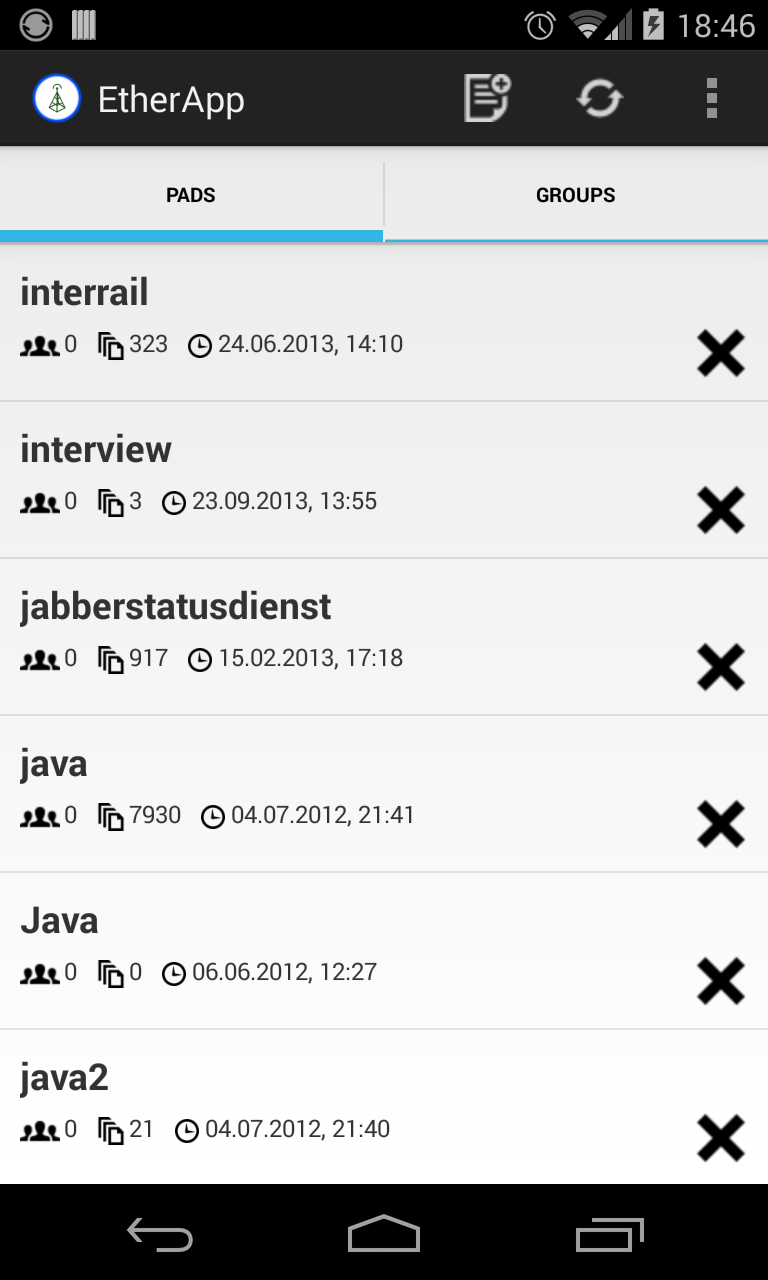
\includegraphics[scale=0.15]{./inc/padliste.png}}
	  \caption{PadlistActivity mit mehreren PadItems}
	  \label{fig:Padliste}
\end{figure}


\subsection{Asynchrones Laden der Listenelemente}
Um eine komplette Padliste inklusive der Metadaten zu jedem Pad abzurufen, sind folgende Anfragen an die HTTP-API nötig:
\begin{itemize}
	\item Abrufen der Padliste (nur IDs)
	\item Abrufen der Metadaten zu jedem einzelnen Pad
		\begin{itemize}
			\item Anzahl der User online
			\item Anzahl der Revisionen
			\item Datum der letzten Bearbeitung
		\end{itemize}
\end{itemize}

Für jedes Pad sind also drei HTTP-Anfragen abzusetzen.
Bei einem Volumen von 300 Pads sind damit 901 HTTP-Anfragen nötig, um alle Daten der Padliste abzurufen, auch wenn der Benutzer diese zunächst gar nicht benötigt!
Neben der dadurch ausgelösten Serverlast ist auch die resultierende Wartezeit für den Benutzer nicht akzeptabel.
Dieser Umstand erfordert eine Lösung, mit der die Inhalte eines Listenelements erst dann geladen werden, wenn das Element auch angezeigt wird.\\
Dieses Ziel kann mit einem \texttt{AsyncTask} erreicht werden.
Zunächst wird die Liste aller Pads abgerufen und das \texttt{ListView} mit Elementen gefüllt. Jedes angezeigte Listenelement startet dann einen neuen Thread (\texttt{AsyncTask}) für jeden zu ladenden Wert.
Der Thread stellt asynchron eine Anfrage an die API und schreibt die Ergebnisse direkt in die Views des Listenelements.
Das asynchrone Laden ist beim Scrollen der Liste an der Zeitverzögerung zu erkennen.

\newpage
\subsection{Verwaltung mehrerer EPL-Instanzen}
\label{sub:implem:eplinstanzen}
Zur Verwaltung mehrerer Instanzen des EPL auf verschiedenen Servern wurde eine Profilverwaltung implementiert.
Die benötigten Informationen für den Zugriff auf eine EPL-Instanz sind in \autoref{tbl:EPLi} zu sehen.
In den Einstellungen können Daten für verschiedene APIs eingetragen werden.
Jeweils eine API kann zur Verwendung ausgewählt werden.
Beim Start der App wird die zuletzt ausgewählte API verwendet.
Startet die App zum ersten Mal, wird der Benutzer direkt zum Anlegen einer neuen API aufgefordert.

\begin{table}[h!]
    \begin{center}
      \footnotesize
      \begin{tabular}{|l|l|}
          \hline \textbf{Information} & \textbf{Beschreibung}\\
          \hline
          \hline API-Name & eindeutiger Name einer EPL-Instanz\\
          \hline URL & Adresse der API\\
          \hline Port & verwendeter Port\\
          \hline API-Key & geheimer Schlüssel für den Zugriff\\
          \hline
      \end{tabular}
    \caption{Benötigte Informationen für eine EPL-Instanz}
    \label{tbl:EPLi}
    \end{center}
\end{table}

\subsection{Persistenter Datenspeicher}
Einige Parameter der EtherApp müssen persistent gespeichert werden, z.B. die vom Benutzer definierten APIs und Grundeinstellungen.
Für diese Aufgabe gibt es zwei\\
Lösungsansätze: Shared Preferences und eine SQLite-Datenbank.

Die \textbf{Shared Preferences} sind Schlüssel-Wert-Paare, auf die systemglobal von Applikationen zugegriffen werden kann.
Da uns die Implementation einfacher erschien, sollte diese Methode zum Speichern der API-Informationen verwendet werden.
Dazu wurde dem Schlüssel (z.B. \texttt{apikey}) ein Index angefügt (z.B. \texttt{apikey2}) um die Zugehörigkeit zu einer API-Einstellung, die aus mehreren Schlüsseln besteht, erkennbar zu machen.
Diese Variante funktionierte, hatte aber ihre Grenzen.
Da es keine Funktion gibt, alle existierenden Schlüssel abzurufen, musste immer die Anzahl der existierenden APIs mitgespeichert werden, um durch die Liste iterieren zu können.
Sobald ein Eintrag gelöscht wurde, traten Konsistenzprobleme auf, die nur mit viel Aufwand wieder zu beheben gewesen wären.
Wir entschieden uns daher für eine Migration auf \textbf{SQLite}, ein leichtgewichtiges relationales Datenbanksystem auf Dateibasis.\\
Android stellt bereits  die nötigen Schnittstellen für SQLite-Datenbanken zur Verfügung.
Die Daten lassen sich mit einer relationalen Datenbank wesentlich leichter auslesen und verändern, obgleich die Implementation und Einrichtung etwas aufwendiger ist, als für die Shared Preferences.\\
Zum Zugriff auf die Datenbank wurde die Klasse \texttt{de.etherapp.sql.DBHandler} als Extension der Elternklasse \texttt{SQLiteOpenHelper} angelegt.
Sie stellt die Datenbank für den Schreib- oder Lesezugriff zur Verfügung und regelt die Initialisierung der Datenbank beim ersten Start der App oder beim Upgrade.\\
\\
Für die EtherApp wurden zwei Tabellen angelegt.
\texttt{ea\_padapi} beinhaltet alle Parameter für die API-Definition.
Zur Identifizierung eines Datensatzes wird eine interne UUID verwendet.
Die Tabelle \texttt{ea\_pref} nimmt Schlüssel-Wert-Paare für verschiedene Einstellungen auf, z.B. die UUID der zuletzt ausgewählten API.\\
Die Struktur der Datenbanktabellen ist nachfolgend dargestellt.

\begin{table}[h!]
	\begin{center}
		\footnotesize
		\begin{tabular}{|p{2.5cm}|p{3.5cm}|p{3cm}|}
			\hline
			\multicolumn{3}{|c|}{\textbf{ea\_padapi}} \\ \hline
			\hline
			apiid 	& VARCHAR(64) 	& PRIMARY KEY \\ \hline
			apiname	& VARCHAR(255) 	& NOT NULL \\ \hline
			apiurl 	& VARCHAR(255) 	& NOT NULL \\ \hline
			port	& INT 			& NOT NULL \\ \hline
			apikey	& VARCHAR(255)	& NOT NULL \\ \hline
			timestamp & UNIX\_TIMESTAMP	&  \\ \hline
		\end{tabular}
	\end{center}
\end{table}

\begin{table}[h!]
	\begin{center}
		\footnotesize
		\begin{tabular}{|p{2.5cm}|p{3.5cm}|p{3cm}|}
			\hline
			\multicolumn{3}{|c|}{\textbf{ea\_pref}} \\ \hline
			\hline
			name 	& VARCHAR(255) 	& PRIMARY KEY \\ \hline
			value 	& VARCHAR(255) 	& NOT NULL \\ \hline
		\end{tabular}
	\end{center}
\end{table}


\subsection{TabActivity}
Zur Navigation zwischen den Haupt-Activities (Padliste, Gruppenliste, ...) entschieden wir uns für eine Tab-Ansicht.
Am oberen Rand des Bildschirms sollte eine Tab-Leiste zu sehen sein, beim Anklicken sollte der Inhaltsbereich unten aktualisiert werden (siehe \autoref{fig:tabactivity}).\\
Für diesen Zweck ist das View-Element \texttt{TabHost} entwickelt worden.
Innerhalb einer \texttt{TabActivity} sorgt es für die Auslieferung von Tabs.
Es stellt einen Rahmen zur Verfügung, in den je nach aktivem Tab eine Activity geladen wird.\\
Später fiel uns auf, dass dieses Feature als \textit{deprecated} eingestuft ist und nicht mehr verwendet werden soll.
Stattdessen sollen Tab-Ansichten mit sogen. Fragments implementiert werden.
Die Migration auf eine Fragment-Umgebung hätte jedoch eine vollkommene Umstrukturierung der Software mit sich gebracht und wurde aus Zeitgründen nicht durchgeführt.

\begin{figure}[h!]
    \centering
    \setlength\fboxsep{0pt}
    %\setlength\fboxrule{0.5pt}
    \fbox{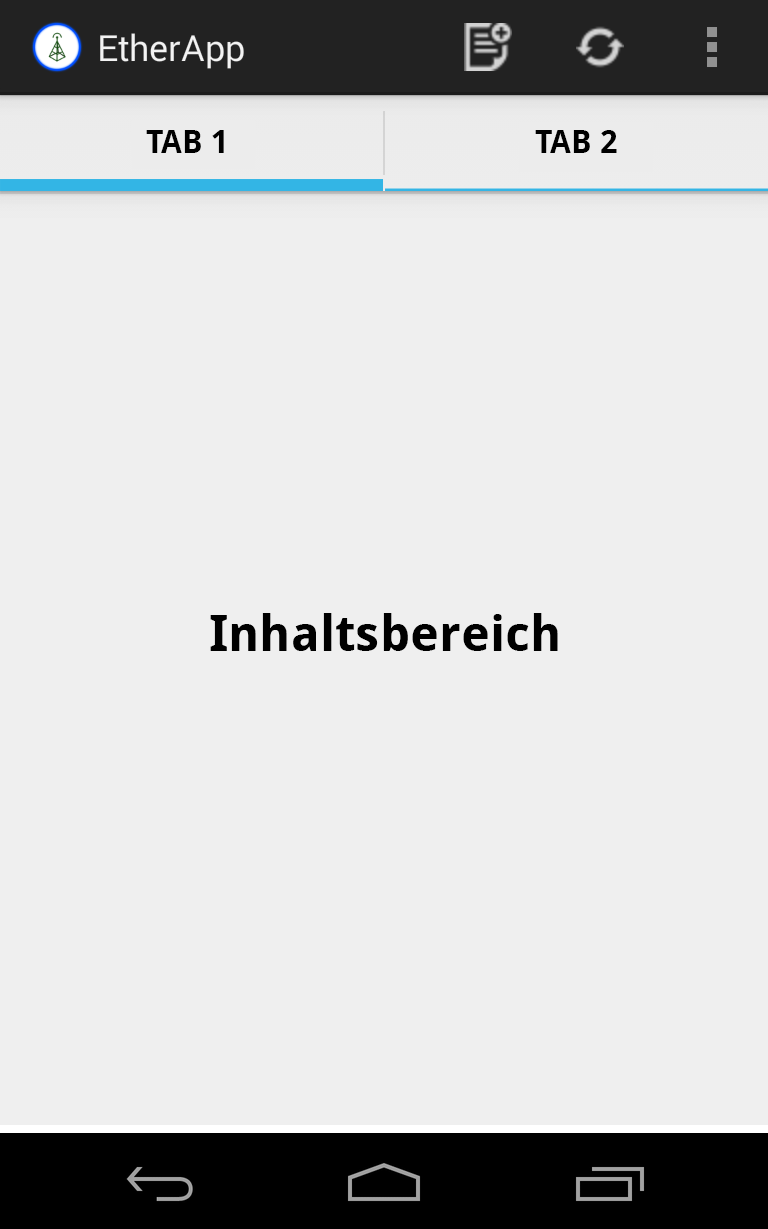
\includegraphics[scale=0.20]{./inc/tabactivity.png}}
	  \caption{TabActivity mit Tabs und Inhaltsbereich}
	  \label{fig:tabactivity}
\end{figure}

\newpage
\subsection{Datenstruktur}
Alle Daten (APIs, Pads, Gruppen) der EtherApp werden in einer Klassenstruktur gespeichert. Die gesamte Struktur ist in \autoref{fig:klassendiagramm} dargestellt.\\
Die Wurzel der Struktur ist die statische Klasse \texttt{GlobalConfig}.
Sie enthält eine \texttt{HashMap} mit allen angelegten APIs, jeweils Objekte der Klasse \texttt{PadAPI}.
Innerhalb der API beinhaltet eine \texttt{HashMap} alle Pads inklusive ihrer Parameter (sofern schon abgerufen).
Ein Pad ist in einem Objekt der Klasse \texttt{Pad} repräsentiert.\\
In der \texttt{GlobalConfig} sind außerdem der \texttt{DBHandler}, die \texttt{MainActivity} (Host für die Tab-Ansicht) und die aktuell ausgewählte API als Objekte hinterlegt.\\
Die Klasse \texttt{PadThread} ruft beim Start die komplette Liste aller Pads asynchron aus der API ab.

\begin{figure}[h!]
    \centering
    \setlength\fboxsep{0pt}
    %\setlength\fboxrule{0.5pt}
    \fbox{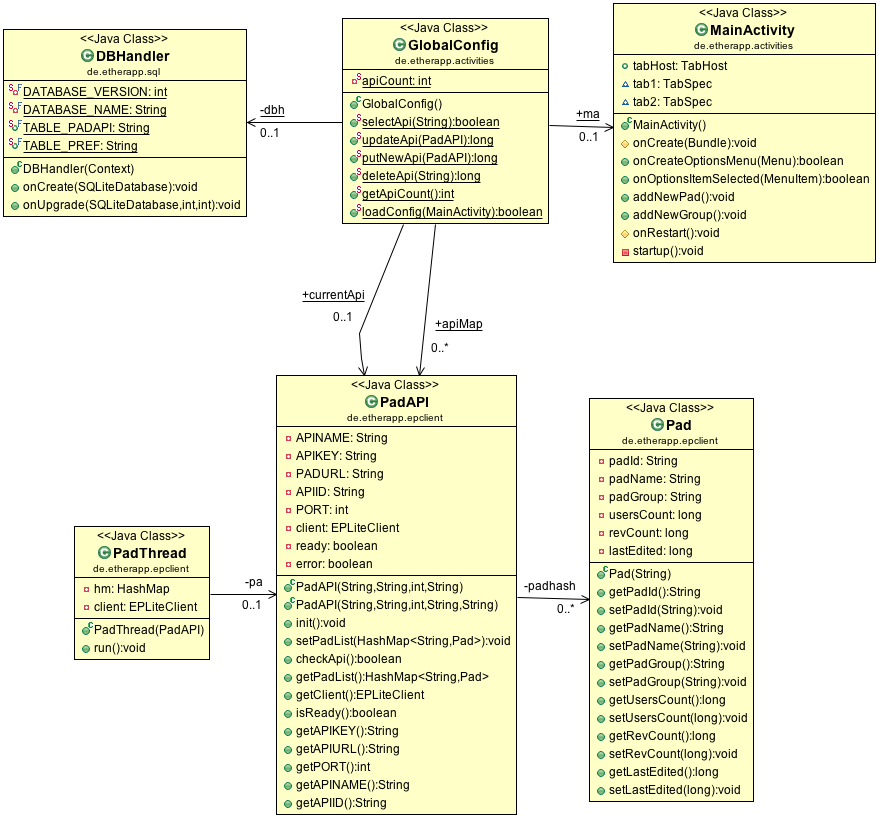
\includegraphics[scale=0.45]{./inc/etherapp_classes.png}}
	  \caption{Klassendiagramm der EtherApp}
	  \label{fig:klassendiagramm}
\end{figure}


\section{Probleme bei der Umsetzung}
Hinsichtlich des Software-Engineering-Prozesses wurde das Modell des Extreme Pair Programming mit Rapid Prototyping verfolgt.
Die Implementation erfolgte zum großen Teil gemeinschaftlich, mit dem Ziel, einen schnellen Prototypen zu entwickeln.
Dieses Vorgehen und der Umstand, dass wir uns das weite Feld der Software-Entwicklung auf einer Android-Plattform erst erschließen mussten, führten zu Unsicherheiten in der Umsetzung.\\
Die bestehenden Konzepte wurden mehrfach überarbeitet und an gewonnene Erkenntnisse angepasst.
Viele Eigenschaften, die noch zu Beginn des Entwicklungsprozesses sinnvoll erschienen, erwiesen sich später als überflüssig.\\
Einige Problemstellungen sind nachfolgend kurz beschrieben.

\subsection{Asynchrone Netzwerkkommunikation}
Aus der Theorie ist bekannt, dass blockierende Netzwerkaufrufe nicht im Hauptthread der Anwendung durchgeführt werden sollten, da die gesamte Anwendung (und damit auch das UI) dann blockiert.
An einigen Stellen (z.B. beim Starten der App und dem initialen Laden der Padliste) kann ein Benutzer eine Wartezeit allerdings in Kauf nehmen.\\
Der Einfachheit halber (und weil diese Eigenschaft die Bedienbarkeit der App nicht in hohem Maße einschränkt), sollten die meisten Netzwerkaktionen synchron im Hauptthread erfolgen.
Android verbietet in der Default-Konfiguration jedoch Netzwerkzugriff im Hauptthread (\texttt{android.os.NetworkOnMainThreadException}).\\
Teilweise konnten wir die Netzwerkaktionen auf Threads auslagern (\texttt{PadThread} zum Abrufen der Padliste ohne Metadaten oder \texttt{Asynctask}s für Metadaten der Pads).
Einfache Threads haben allerdings dann ihre Grenzen, wenn die Daten direkt in ein \texttt{View}-Element geschrieben werden sollen.
Einzelne Versuche, die Funktionalität mit Services zu implementieren, scheiterten.\\
Daher entschieden wir uns schlussendlich, Netzwerk auf dem MainThread zu erlauben, obgleich dieses Vorgehen nicht unbedingt der \textit{best practice} entspricht.
Perspektivisch sollten alle Netzwerkzugriffe über einen \texttt{AsyncTask} ausgeführt werden.

\subsection{Fehlerbehandlung}
Erst während der Implementation fiel uns auf, wie umfangreich die Fehlerbehandlung bei einer Applikation sein kann, die Daten aus einer anderen Quelle bezieht und nicht nur in sich geschlossen arbeitet.
Jeder Netzwerkaufruf kann durch verschiedene Faktoren beeinflusst werden:
\begin{itemize}
	\item Ist der Internetzugriff aktiviert? (WLAN, GPRS, UMTS)
	\item Darf die App auf das Internet zugreifen? (Firewall)
	\item Ist der Verbindungsaufbau überhaupt möglich? (Netzempfang, Störungen auf der Strecke)
	\item Ist der EPL-Server verfügbar?
	\item Sind die API-Daten korrekt?
\end{itemize}

In den ersten Iterationen des Projekts wurden diese Punkte in keiner Weise berücksichtigt und vorerst auf den Idealfall vertraut.
Nachdem wir feststellen konnten, dass die App bei jedem Fehler aber sofort abstürzt, nahmen wir die Fehlerbehandlung als \textit{must-have} bis zum ersten Release auf.
Dabei beschränkten wir uns darauf, die Konnektivität und erfolgreiche Authentifizierung an der API zu prüfen.

\subsection{Umlaute in Pad-ID}
Die App generiert Fehler, sobald in einer Pad-ID Umlaute oder Sonderzeichen auftreten; das EPL selbst und seine API unterstützen Umlaute jedoch problemlos.
Die Vermutung fiel schnell auf das URL-Encoding der übergebenen ID.
Einzelne Versuche führten allerdings zu keinem Erfolg.
Leider konnten wir den Fehler nicht weiter eingrenzen und vertrauen vorerst auf den erfahrenen Pad-Benutzer, der Pads ohnehin nur mit alphanumerischen Zeichen anlegt.

\subsection{Handling von Activities}

